\documentclass[aspectratio=169]{beamer}
\usetheme{Bruno}
\usepackage{amsmath}
\usepackage{amssymb}
\usepackage{siunitx}
\usepackage{float}
\usepackage{tikz}
\def\checkmark{\tikz\fill[scale=0.4](0,.35) -- (.25,0) -- (1,.7) -- (.25,.15) -- cycle;} 
\usepackage{url}
\usepackage[siunitx,american,RPvoltages]{circuitikz}
\ctikzset{capacitors/scale=0.7}
\ctikzset{diodes/scale=0.7}
\usepackage{tabularx}
\newcolumntype{C}{>{\centering\arraybackslash}X}
\renewcommand\tabularxcolumn[1]{m{#1}}% for vertical centering text in X column
\usepackage{tabu}
\usepackage[spanish,es-tabla,activeacute]{babel}
\usepackage{babelbib}
\usepackage{booktabs}
\usepackage{pgfplots}
\usepackage{hyperref}
\hypersetup{colorlinks = true,
            linkcolor = black,
            urlcolor  = blue,
            citecolor = blue,
            anchorcolor = blue}
\usepgfplotslibrary{units, fillbetween} 
\pgfplotsset{compat=1.16}
\usepackage{bm}
\usetikzlibrary{arrows, arrows.meta, shapes, 3d, perspective, positioning}
\renewcommand{\sin}{\sen} %change from sin to sen
\usepackage{bohr}
\setbohr{distribution-method = quantum,insert-missing = true}
\usepackage{elements}
\usepackage{verbatim}
\usetikzlibrary{mindmap,trees,backgrounds}
 
\definecolor{color_mate}{RGB}{255,255,128}
\definecolor{color_plas}{RGB}{255,128,255}
\definecolor{color_text}{RGB}{128,255,255}
\definecolor{color_petr}{RGB}{255,192,192}
\definecolor{color_made}{RGB}{192,255,192}
\definecolor{color_meta}{RGB}{192,192,255}
\usepackage[edges]{forest}
\usepackage{etoolbox}
\usepackage{schemata}
\newcommand\diagram[2]{\schema{\schemabox{#1}}{\schemabox{#2}}}
\title{Instrumentación II: \\ \emph{Adquisición de}\\ \emph{datos}}
\author{Juan J. Rojas}
\institute{Instituto Tecnológico de Costa Rica}
\date{\today}
\background{fig/comunes/background.jpg}
\begin{document}
% \sisetup{unit-math-rm=\mathrm,math-rm=\mathrm} % change sinitx font
\sisetup{output-decimal-marker = {,}}
\maketitle

\newcommand{\blackandwhite}{white} %change this at the end

\begin{frame}{Sistema de adquisición de datos}
\begin{center}
    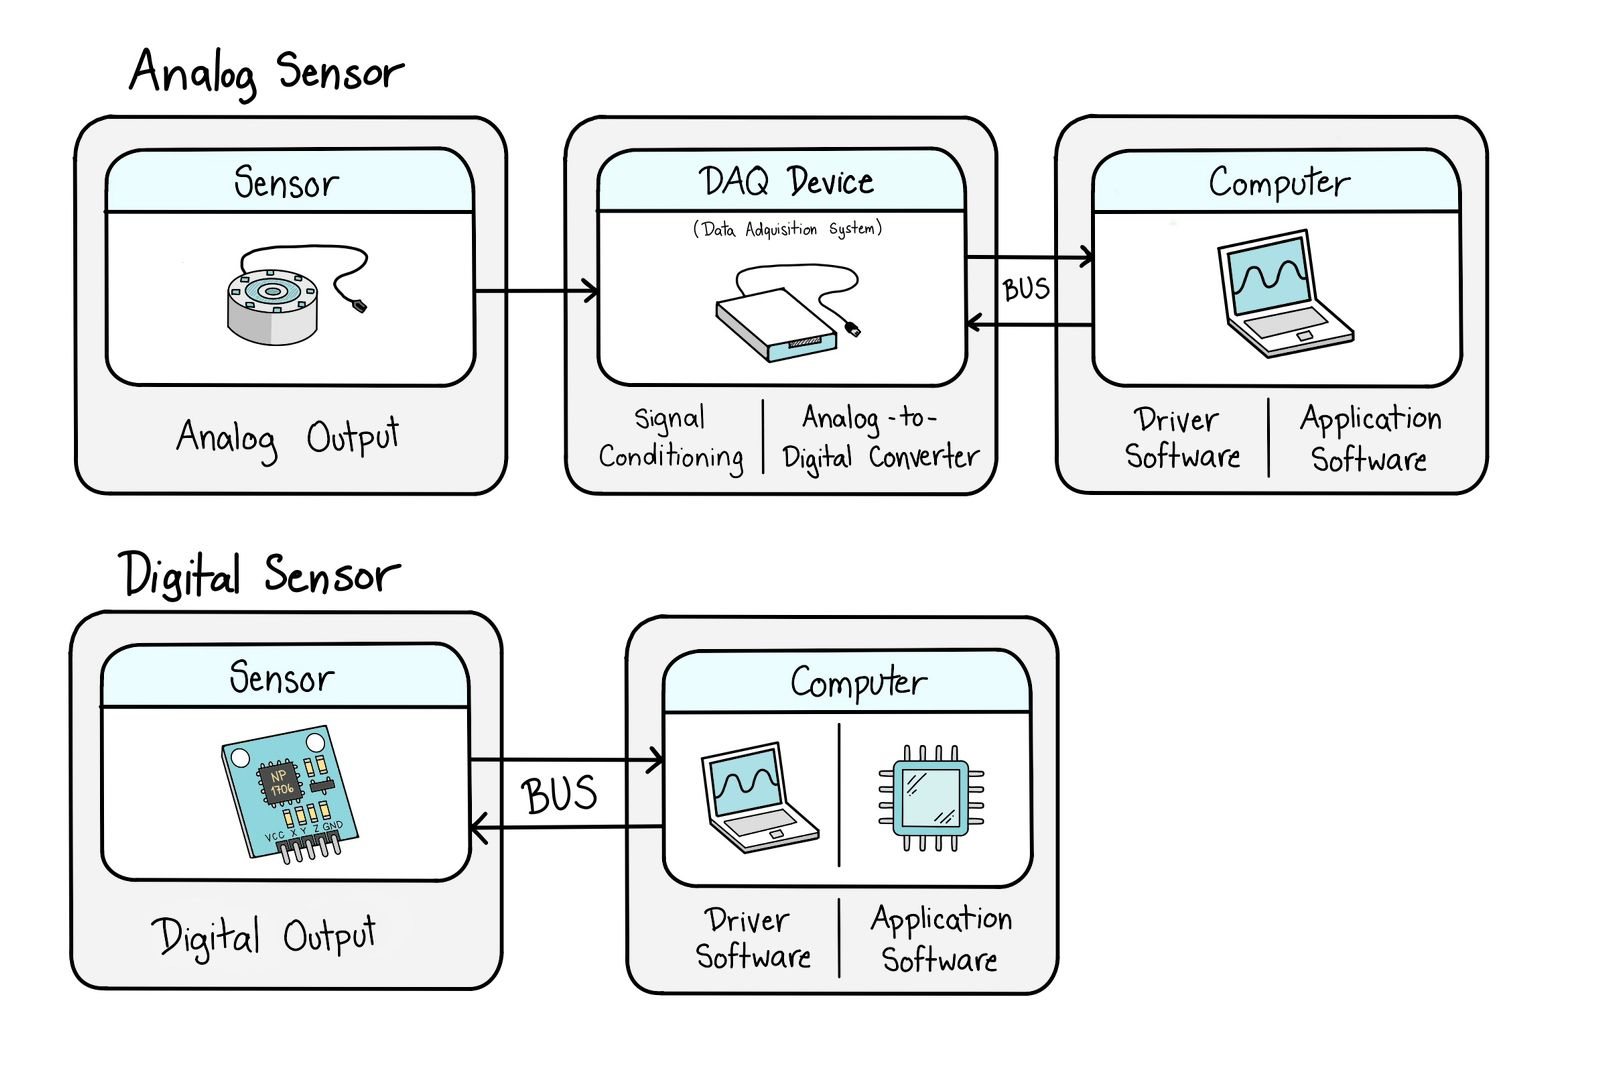
\includegraphics[width=0.93\linewidth]{presentaciones/fig/daqs.jpg}
\end{center}
\end{frame}

\begin{frame}{Señales}
\begin{center}
    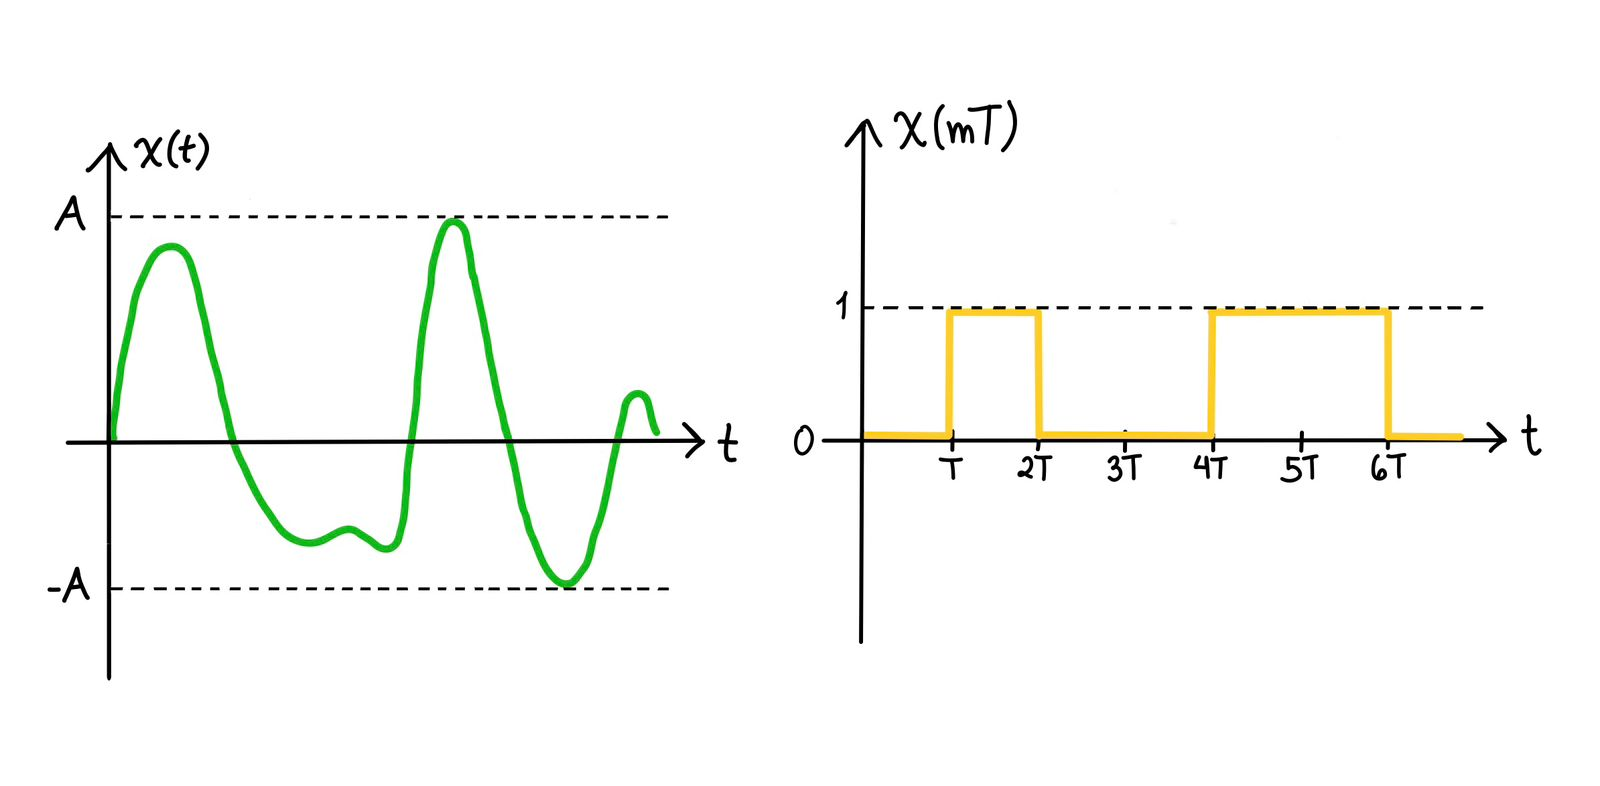
\includegraphics[width=0.8\linewidth]{presentaciones/fig/analogicavrsdigital.jpg}
\end{center}
\end{frame}

\begin{frame}{Etapas de la conversión A/D}
\begin{center}
    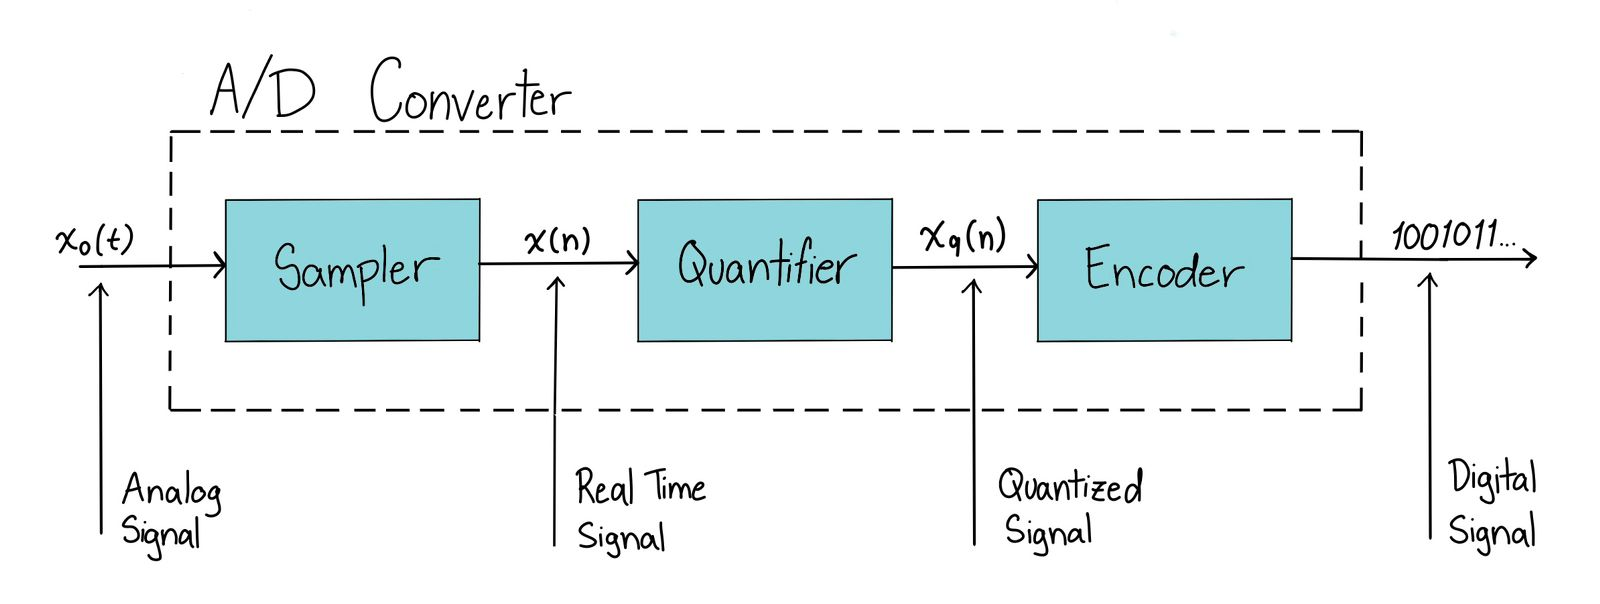
\includegraphics[width=0.93\linewidth]{presentaciones/fig/convAD.jpg}
\end{center}
\end{frame}

\begin{frame}{Muestreo, cuantización y codificación}
\begin{center}
    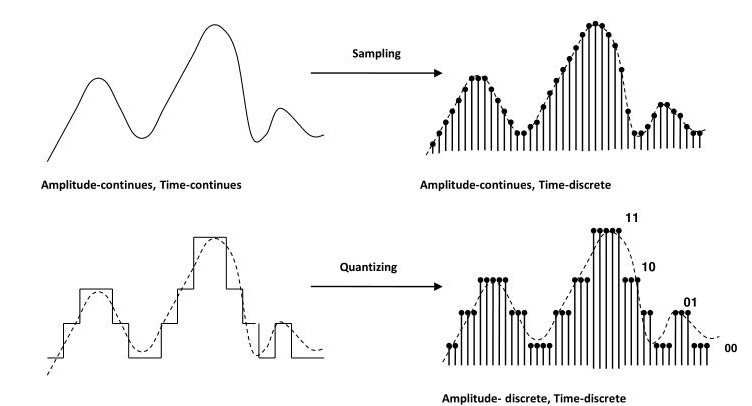
\includegraphics[width=0.9\linewidth]{presentaciones/fig/muestreo.jpg}
\end{center}
\end{frame}

\begin{frame}{Muestreo}
    \begin{columns}
    \begin{column}{0.4\textwidth}
        \centering
        Frecuencia de Nyquist
        \begin{equation*}
            f_N \geq 2\cdot f_{max} 
        \end{equation*}
        una frecuencia de muestreo muy baja puede causar una reconstrucción inexacta de la forma de onda
    \end{column}
    \begin{column}{0.6\textwidth}
        \begin{center}
            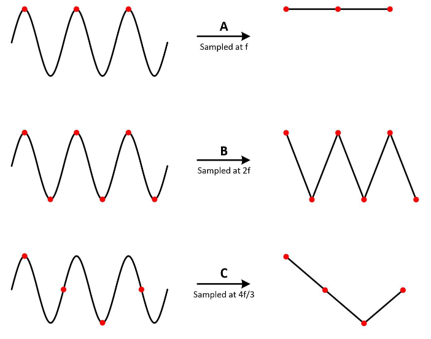
\includegraphics[width=0.9\linewidth]{presentaciones/fig/sampling.png}  
        \end{center}
    \end{column}
    \end{columns}
\end{frame}

\begin{frame}{Cuantización}
    \begin{columns}
    \begin{column}{0.4\textwidth}
        \centering
        Resolución
        \begin{equation*}
            \Delta = \dfrac{\mathrm{Rango}}{2^b-1} 
        \end{equation*}
        Error de cuantización
        \begin{equation*}
            |e_q| \leq \dfrac{\Delta}{2} 
        \end{equation*}
    \end{column}
    \begin{column}{0.6\textwidth}
        \begin{center}
            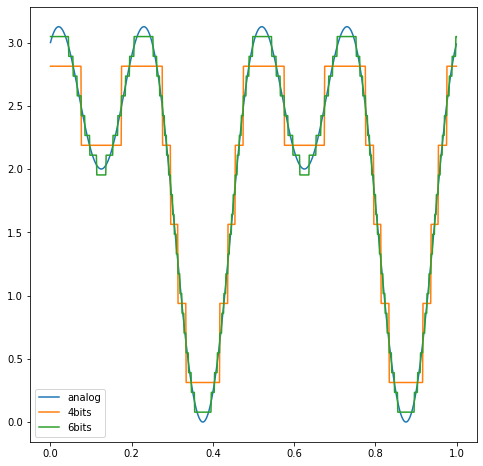
\includegraphics[width=0.8\linewidth]{presentaciones/fig/resolution.png}  
        \end{center}
    \end{column}
    \end{columns}
\end{frame}


\begin{frame}{Ejemplo: aproximación sucesiva}
\begin{center}
    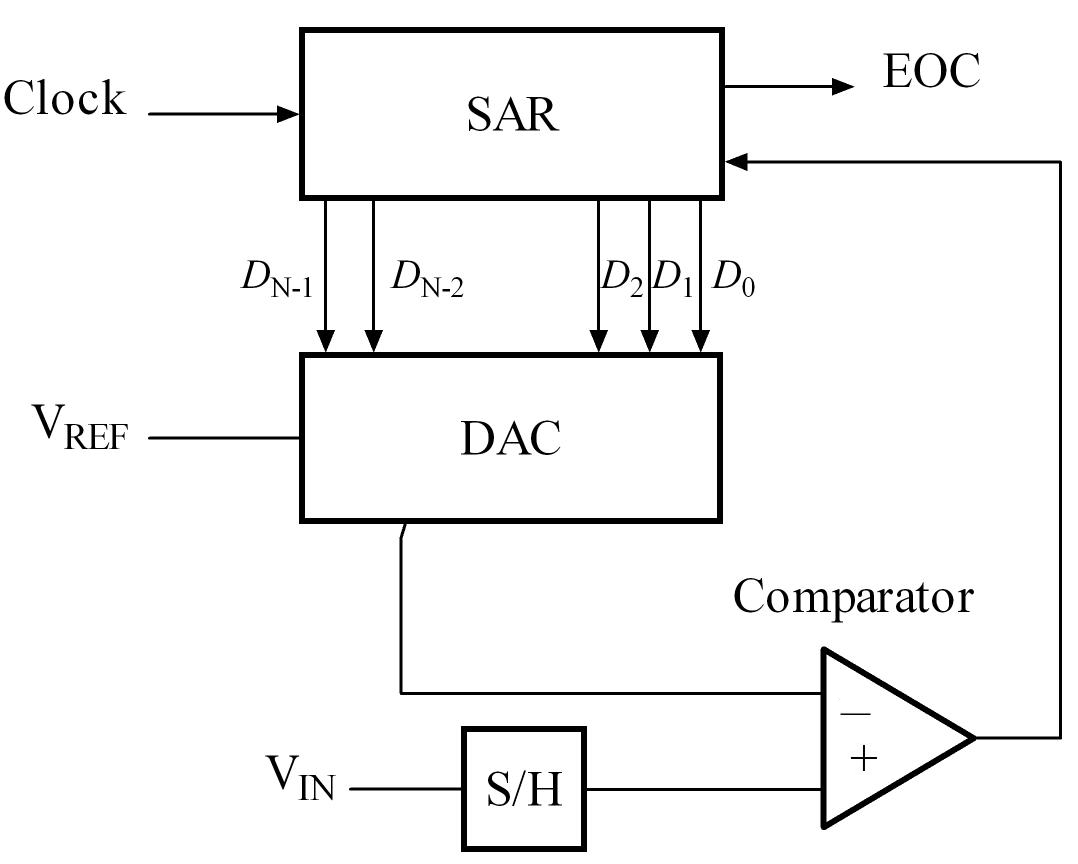
\includegraphics[width=0.5\linewidth]{presentaciones/fig/SAR.png}

\end{center}
{\footnotesize
Sinha, Aritra and Sunit Kumar Sen. “Design of an improved successive approximation type ADC using multi bit per cycle algorithm for conversion rate improvement.” Proceedings of The 2014 International Conference on Control, Instrumentation, Energy and Communication (CIEC) (2014): 219-223.}
\end{frame}

\begin{frame}{Ejemplo: aproximación sucesiva}
    \begin{minipage}[t]{0.45\textwidth}
        \centering
        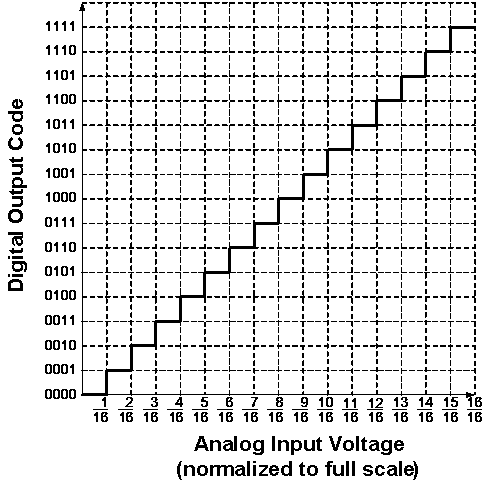
\includegraphics[width=0.9\textwidth]{presentaciones/fig/curve4bit.png}
    \end{minipage}
    \hfill
    \begin{minipage}[t]{0.45\textwidth}
        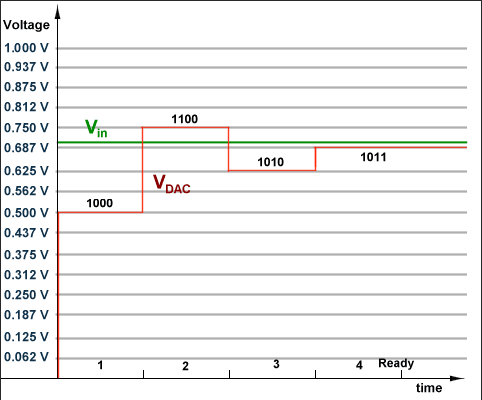
\includegraphics[width=\textwidth]{presentaciones/fig/ADCtime.png}
    \end{minipage}
\end{frame}

% \begin{frame}{Referencias}

% \bibliographystyle{ieeetr}
% \footnotesize
% \bibliography{comunes/referencias}

%\end{frame}

\end{document}